\section{GPU Parallelization}
\textbf{GPU:} extreme data parallelism, simple logic (no branching) but many cores, small caches per core \\
\textbf{CPU:} low data parallelism, branching logic, thread synchronisation, few but powerful cores, large caches per chip

\subsection{Perfomance Analysis}
\textbf{Arithmetic Intensity:} measure of the code in \textbf{FL}oating point \textbf{OP}eration per Byte ratio. the higher, the more efficient the program will run on GPU. 
\[ ArithmeticIntensity = \frac{operations/s}{bytes/s} = \frac{FLOPs}{Bytes} \]

There is a tradeoff between \textbf{Latency:} time a task takes to finish, and \textbf{Throughput:} number of tasks completed in a given timeframe. Increasing throughput can increase the latency of one single workload.

Example calculation: using code 
\texttt{for(i=0;i<N;++i) { z[i] = x[i] + y[i] * x[i]}}
we need to: copy x and y to GPU, z to CPU, assuming size of x,y,z to be 4 bytes
\#arithmetic ops: 2, \#bytes transferred: 12, arithmetic intensity: 2/12 = 1/6

\textbf{Roof Line Model}\\
Compares Peak Performance/Peak Bandwidth to Arithmetic Intensity
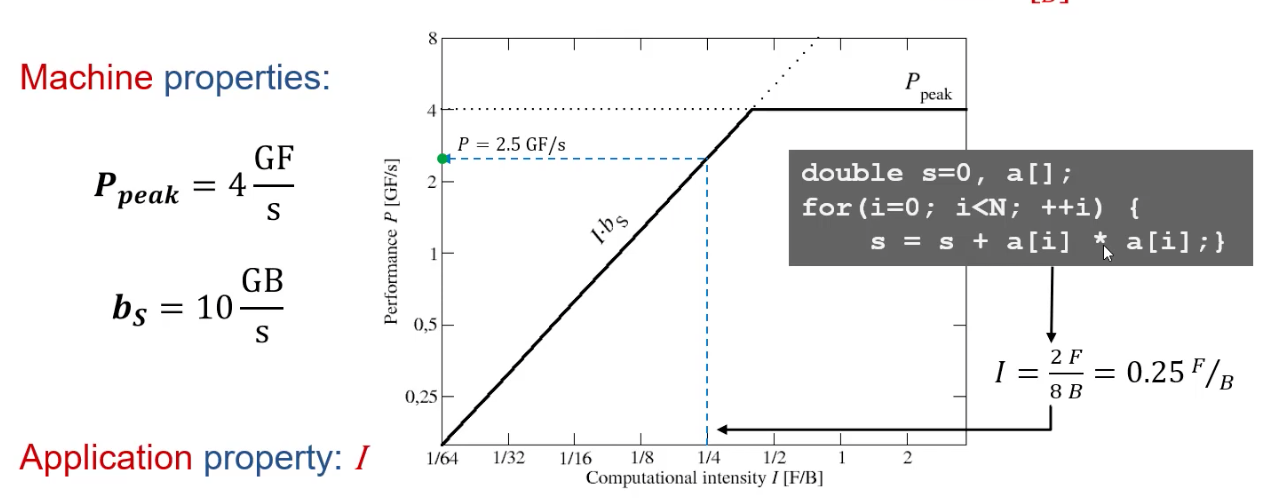
\includegraphics[width=\linewidth]{rooflinemodel.png}

\textbf{Amdahls Law}\\
T = Total time, p = parallel part, $T_n$ = parallel total time, N = number of processors
\begin{minipage}[t]{0.5\linewidth}
  \vspace{-2mm}
  \[ T = (1-p) * T + T_p \]
\end{minipage}
\begin{minipage}[t]{0.5\linewidth}
  \vspace{-2mm}
	\[ SpeedUp = \frac{1}{(1-p) + \frac{p}{N}} \]
\end{minipage}

\subsection{GPU: physical view}

\begin{description}
  \item[GPU Core]= Streaming Processor (SP), many are grouped into a Streaming Multiprocesser (SM, 8-192 SP per SM)
  \item[Shared Memory] per block, access: \texttt{\_\_shared\_\_ float x;}, fast (about 4 cycles), several KB
  \item[Global Memory] main GPU memory,	access: \texttt{cudaMalloc()}, slow (about 400-600 cycles to access), visible to all threads, several GB
  \item[Local Memory] Per thread (spill over), in global memory, only for one thread
  \item[SIMD] Single Instruction Multiple Data (vector-parallelism). All threads run the same kernel code with different data. Only distinction possible are the \texttt{threadId/blockID} builtin variables. 
  \item[Divergence] In branching in code, the instructions are executed only by some threads, others are waiting.
  
  \item[NUMA-Model] Non-uniform memory access. Memory is not shared between CPU and GPU, explicit transfer is necessary. Also describes cluster architecure - any situation without shared memory.
  
  \item[CUDA] Computer Unified Device Architecture is a general purpose programming model, proprietary for Nvidia GPUs. Device Query using \texttt{cudaGetDeviceProperties()}
  
  \item[CUDA Barriere] \texttt{\_\_syncthreads()} syncs all threads inside of one block. all will wait and continue at the same time. If inside an \texttt{if/else} statemet, two different barriers are necessary!
  \item[Kernel Call Parameters] \lstinline|<< Dg, Db, Ns >>| where 
  \textbf{Dg} (dim3): dimension and size of the grid,
  \textbf{Db} (dim3): dimension and size of each block
  \textbf{Ns} (size\_t): number of bytes in shared memory dynamically allocated per block
  \item[Warp] Threads in blocks are divided into Warps that execute the same instruction. Branches in code waiting = performance loss: prefer \texttt{if (threadIdx.x / 32 > 1)}
  \item[DRAM / Memory Coalescing] read operations on global GPU memory always access 32 bytes - use this for access within the same warp. 
\end{description}

\subsection{CUDA Code Examples}
\textbf{Kernel for Vector Addition}
\begin{lstlisting}[style=csharp]
__global__ void add(float *A, float *B, float *C, int N) {
	int i = blockIdx.x * blockDim.x + threadId.x;
	if (i < N) { C[i] = A[i] + B[i]; } // other threads wait
}
\end{lstlisting}  

\textbf{CUDA Matrix Multiplication}
\begin{lstlisting}[style=csharp]
#include <stdio.h> #include <cuda.h>

const int C_ROWS = 1000; const int C_COLS = 2000; const int A_COLS = 1500;
const int A_ROWS = C_ROWS; const int B_ROWS = A_COLS; const int B_COLS = C_COLS;
const int BLOCK_SIZE = 32; // Memory Coalescing
__global__
void matrixMultKernel(float *A, float *B, float *C) {
	int row = blockIdx.x * blockDim.x + threadIdx.x;
	int col = blockIdx.y * blockDim.y + threadIdx.y;
	if (row < C_ROWS && col < C_COLS) {
		float sum = 0.0f;
		for (int k = 0; k < A_COLS; k++) {
			sum += A[row * A_COLS + k] * B[k * B_COLS + col];
		}
		C[row * C_COLS + col] = sum; } }

void cudaMatrixMult(float *A, float *B, float *C) {
  float *d_A, *d_B, *d_C;
  int sizeA = A_ROWS * A_COLS * sizeof(float); // ...B&C
    // allocate device memory
  handleCudaError(cudaMalloc(&d_A, sizeA)); // ...B&C
    // transfer data to device
  handleCudaError(cudaMemcpy(d_A, A, sizeA, cudaMemcpyHostToDevice)); // ...B
    // create definitions for exeuction
  dim3 threadsPerBlock(BLOCK_SIZE, BLOCK_SIZE);
  dim3 blocksPerGrid((C_ROWS + BLOCK_SIZE - 1) / BLOCK_SIZE, (C_COLS + BLOCK_SIZE - 1) / BLOCK_SIZE);
    // run kernel on device
  matrixMultKernel<<<blocksPerGrid, threadsPerBlock>>>(d_A, d_B, d_C);
  handleCudaError(cudaGetLastError());
    // transfer data from device
  handleCudaError(cudaMemcpy(C, d_C, sizeC, cudaMemcpyDeviceToHost));
    // memory cleanup
  handleCudaError(cudaFree(d_A)); // ...B&C
}
\end{lstlisting}

% TODO Replace example with something understandable..
\textbf{Array Sum up:} this example sums pairs inside an array and adds them in a second step
\begin{lstlisting}[style=csharp]
__global__ void parallelSum(int* array, int length) {
  int offset = blockIdx.x * blockDim.x;
  int stride = 1;
  while (stride < blockDim.x) {
    int first = offset + 2 * stride * threadIdx.x; 
    int second = first + stride;
    if (second < length) {
      array[first] += array[second];
    }
    stride *= 2;      
    __syncthreads();
  }
}
\end{lstlisting}
\textbf{Cuda Error Handling Function}
\begin{lstlisting}[style=csharp]
  void handleCudaError(cudaError error) { 
    if (error != cudaSuccess) { fprintf(stderr, "CUDA: \%s!\n", cudaGetErrorString(error));
    exit(EXIT_FAILURE);    } }
\end{lstlisting}

\subsection{Data Partitioning}
maxThreadsPerBlock: 1024 (total), maxThreadsDim: 512, 512, 64
\begin{lstlisting}[style=csharp]
N = 1000000; int nofBlocks = (N + 1023) / 1024;
VectorAddKernel<<<nofBlocks, 1024>>>(A, B, C, N);
\end{lstlisting}
\vspace{1mm}
\begin{lstlisting}[style=csharp]
dim3 block = (2,2); // no of threads
dim3 grid = (3,2); // no of blocks
VectorAddKernel<<<grid, block>>>(A, B, C);
\end{lstlisting}
\textbf{dim3()}
\begin{lstlisting}[style=csharp]
 __global__ void VectorAddKernel(float *A, float *B, float *C) {
   int row = blockIdx.x * blockDim.x + threadIdx.x;
   int column = blockIdx.y * blockDim.y + threadIdx.y;
   
   if (row < A_ROWS && col < A_COLS) {
      C[row * A_COLS + col] = A[row * A_COLS + col] + B[row * A_COLS + col]; 	}	}
\end{lstlisting}
\subsection{Tiled Matrix Multiplication}
\begin{lstlisting}[style=csharp]
__global__ void matrixMultKernel(float* A, float* B, float* C) {
	__shared__ float Asub[TILE_SIZE][TILE_SIZE];
	__shared__ float Bsub[TILE_SIZE][TILE_SIZE];

	int tx = threadIdx.x, ty = threadIdx.y;
	int col = blockIdx.x * TILE_SIZE + tx;
	int row = blockIdx.y * TILE_SIZE + ty;
	int nofTiles = (A_COLS + TILE_SIZE - 1) / TILE_SIZE;

	float temp = 0.0;

	for (int tile = 0; tile < nofTiles; tile++) {
		if (row < A_ROWS && tile * TILE_SIZE + tx < A_COLS) {
			Asub[ty][tx] = A[row * A_COLS + tile * TILE_SIZE + tx];
		} else { Asub[ty][tx] = 0; }

		if (col < B_COLS && tile * TILE_SIZE + ty < B_ROWS) {
			Bsub[ty][tx] = B[(tile * TILE_SIZE + ty) * B_COLS + col];
		} else { Bsub[ty][tx] = 0; }
		__syncthreads();
		if (row < C_ROWS && col < C_COLS) {
			for (int k = 0; k < TILE_SIZE; k++) {
				if (tile * TILE_SIZE + k < A_COLS) {
					temp += Asub[ty][k] * Bsub[k][tx];
		} } }
		__syncthreads();
		if (row < C_ROWS && col < C_COLS) {
			C[row * C_COLS + col] = temp;
} } }
\end{lstlisting}